\section{Multi-Leader репликация. Last Write Wins.}
    Один из способов решения конфликта - оставлять на каждой реплике только последнюю (в некотором смысле) запись. Нельзя на каждой реплике сохранять последнюю пришедшую запись, потому что тогда, они даже eventually не придут к согласованности. \\
    Решения:
    \begin{itemize}
        \item физические часы - каждая запись будет иметь метку времени - физическое время той реплики, которая приняла эту запись, но из-за плохо синхронезированных часов может отбросить последнюю запись, хотя последнюю надо оставлять.
        \item логические часы - векторные часы, основанные на отношении "произошло до", но среди паралельных записей нет той, которая произошла до, и брать любую из них тоже нельзя.
    \end{itemize}
      \begin{definition}
        Last Write Wins не работает при выборе любой из параллельных записей
      \end{definition}
          $c$ happens-before $b$, $a || b$, $a || c$. \\
          Приоритет по убыванию: $c$, $b$, $a$. \\
          \begin{itemize}
          \item При конфликте берем покомпонентый максимум векторных версий: \\
          $a + c = c, a + c || b$\\
          $(a + c) + b = a + c = c$\\
          $a + b = a, c -> (a + b)$\\
          $(a + b) + c = a + b = a$
          \item При конфликте берем версию победителя: \\
          $a + c = c, (a + c) -> b$ \\
          $(a + c) + b = b$ \\
          $a + b = a, (a + b) || c$\\
          $(a + b) + c = c$
          \end{itemize}
        Поэтому держать только актуальное значение на реплике, и заменять при необходимости на нужное не получится. \\
        Решение - для каждого ключа на каждой реплики храним $N$ значений - последнее полученное с каждой из $N$ реплик значение по соответствующему ключу. \\
        Когда хотим получить актуальное значение, строим множество $W$, в котором оставим только параллельные операции, а те которое связаны хоть с кем-то отношением "произошло до" выкинем, среди этого множествва оставим одно значение произвольным образом, например по timestamp'у.
    Серьезная проблема - понимать, когда и какую из старых операций можно забыть.\\
    \begin{example}
      РСУБД:\\
      \begin{figure}[h]
          \centering
          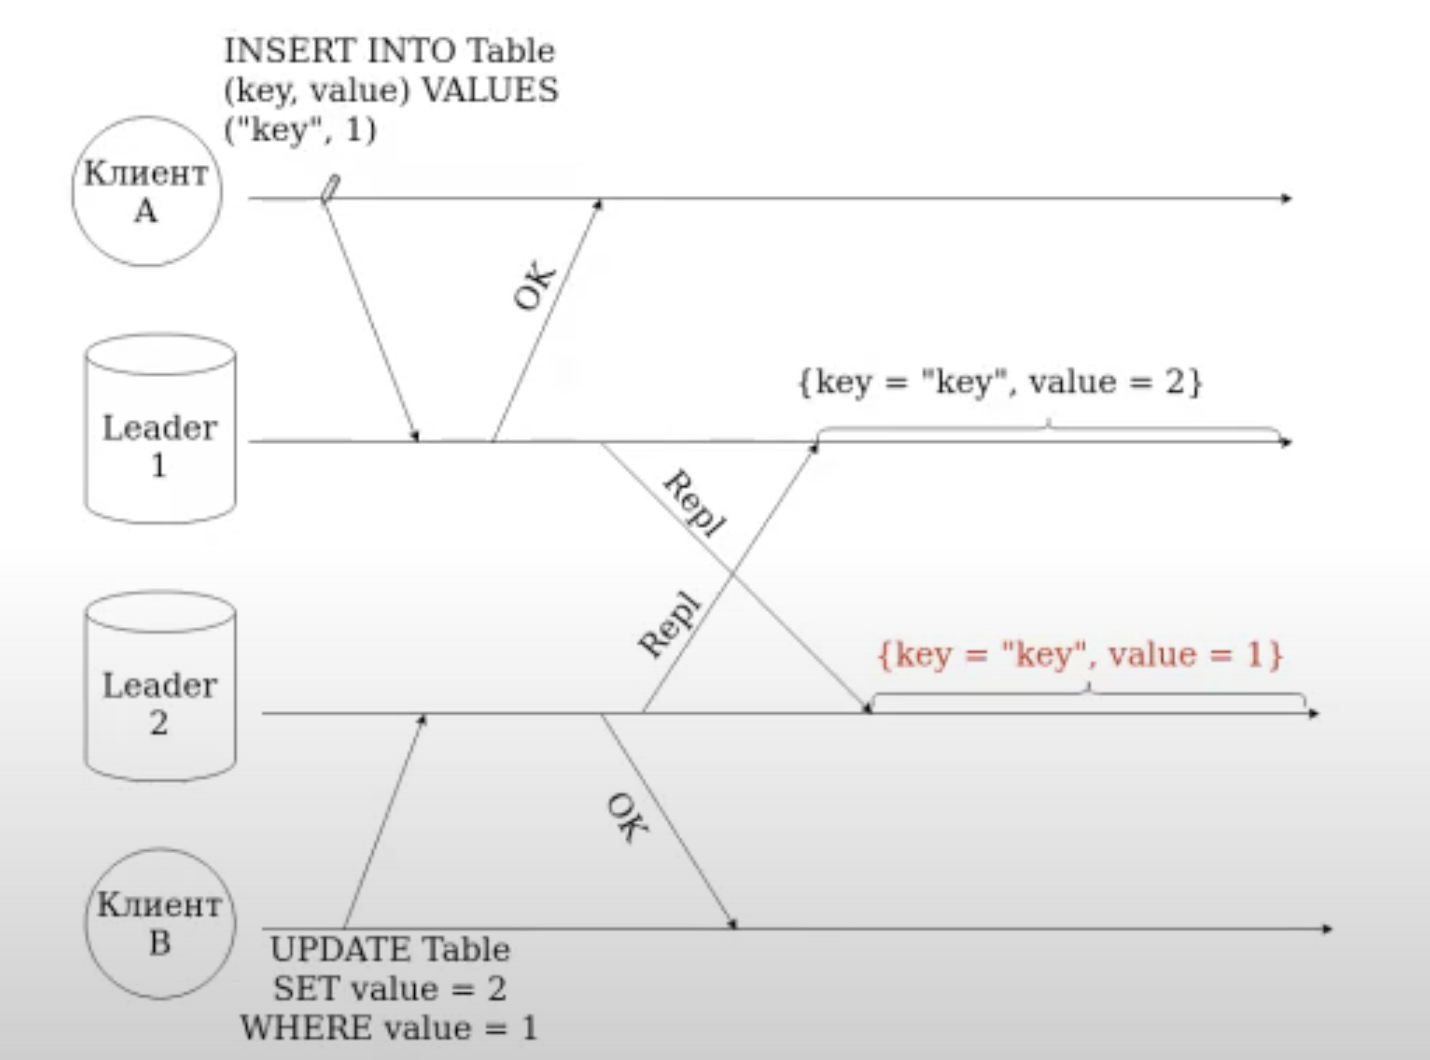
\includegraphics[scale = 0.5]{14.png}
          \caption{Граф - контрпример}
      \end{figure}
      Даже если в операции не упоминается явно ключ - не значит, что можно забыть.\\
    \end{example}
    Проблемы даже с инкрементором.\\
    \begin{definition}
    Инкрементор
    \end{definition}
      Состояние - единственное число.\\
      Система выполняет запросы вида "увеличить число на k"\\
      Если не храним предка пришедшей записи, то мы не можем сказать, на сколько увеличил третий узел.\\
      Решение:\\
      \begin{figure}[h]
          \centering
          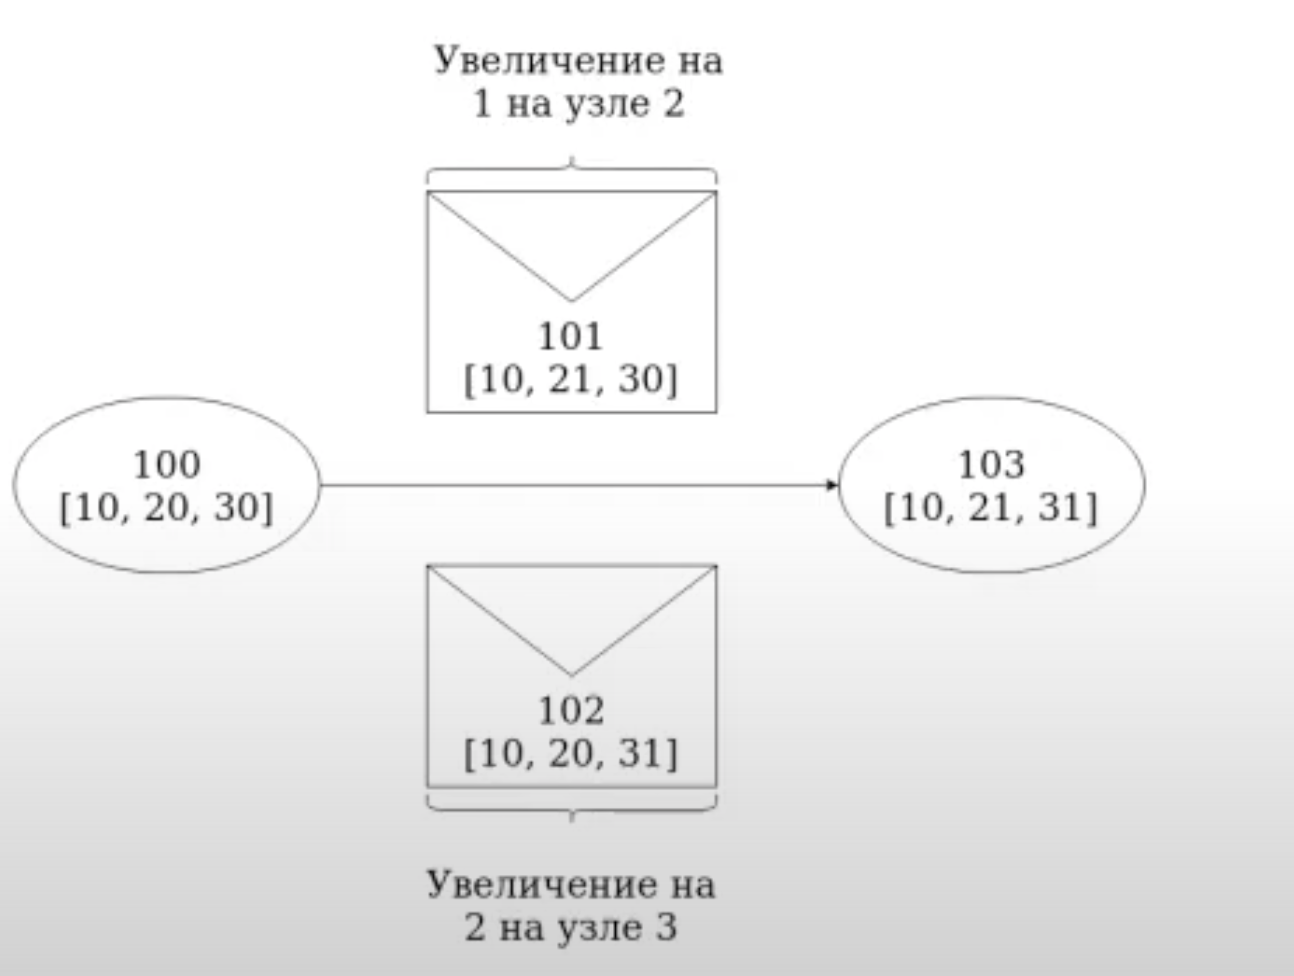
\includegraphics[scale = 0.5]{../assets/15.png}
          \caption{Параллельная запись}
      \end{figure}
      \begin{figure}[h]
          \centering
          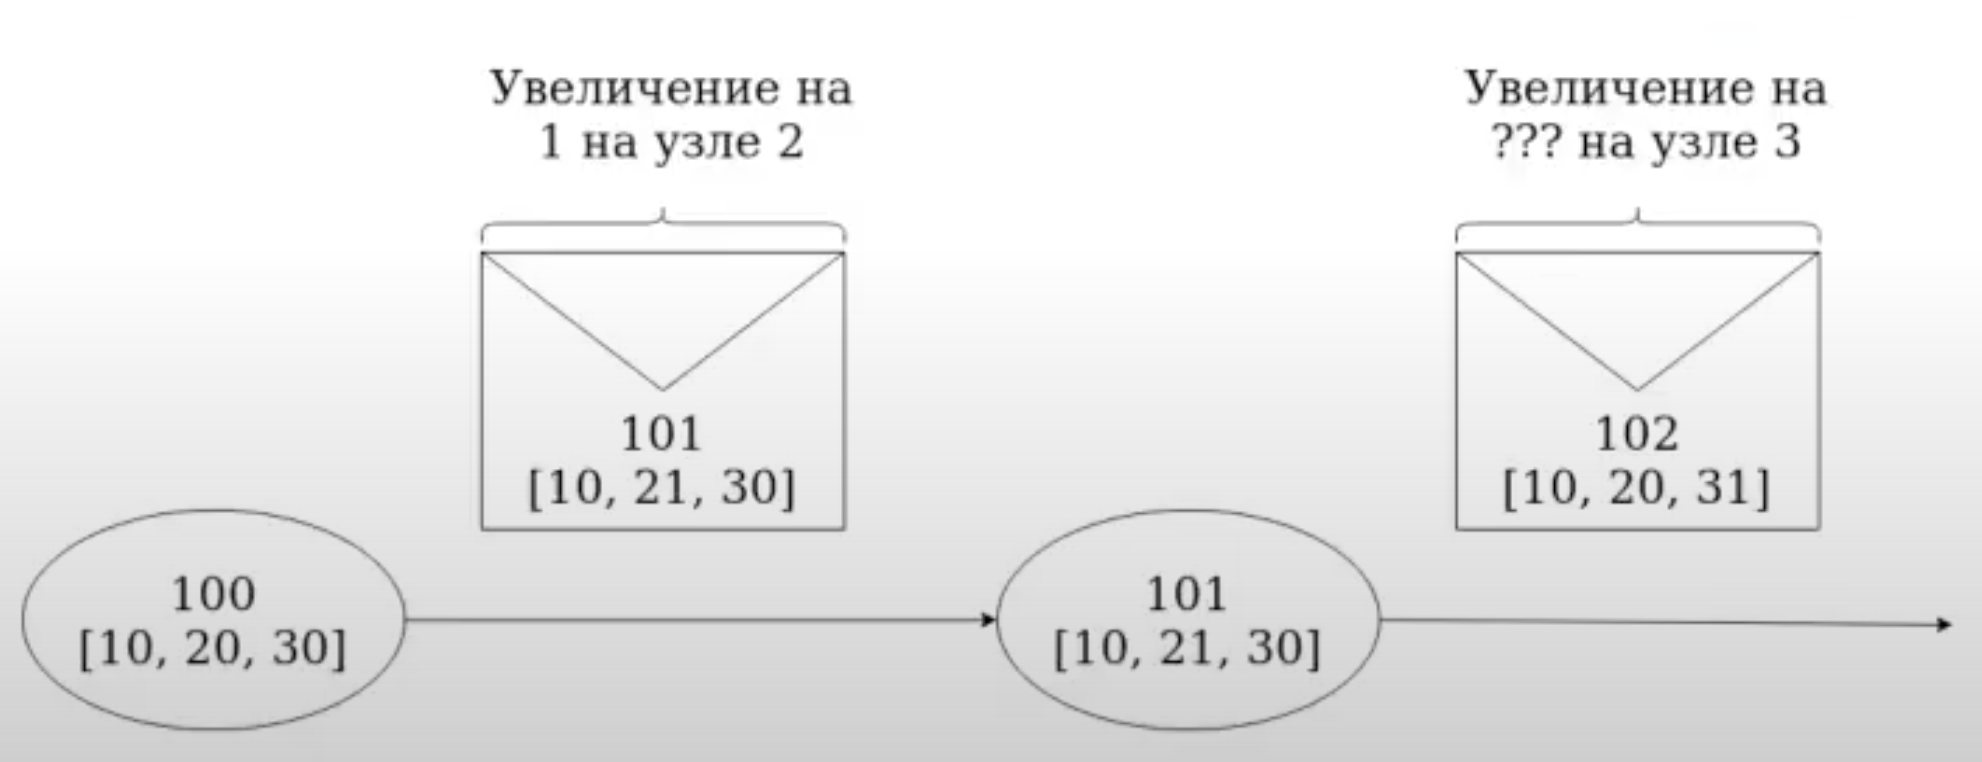
\includegraphics[scale = 0.5]{../assets/16.png}
          \caption{Последовательная запись}
      \end{figure}
      Храним старое состояние, пока имеется возможность получить его непосредственного потомка.\\
      Выкидываем старое, когда по каждой компоненте вектора $V$ получили "следующее" состояние.
